
\chapter{Аналитический раздел}
В данном разделе будет представлен анализ предметной области, проведена формализация задачи, проведена формализация и описание информации для хранения в БД, проведена формализация и описание пользователей и проанализированы модели баз данных. 
\section{Анализ предметной области}
Развитие информационных технологий, помимо различных сфер по всей земле, также не обошло и музыкальную сферу.
Музыкальная индустрия одной из первых ощутила на себе смену технологических эпох, изменившись за последние 20 лет на всех уровнях \cite{music_and_it}.

Российский рынок услуг звукозаписи --- это динамично развивающаяся отрасль, которая с каждым годом приобретает все большую популярность и значимость.
Еще в 2017 году в России было примерно 656 студий звукозаписи, а в 2023 году их насчитывалось около 1160 студий звукозаписи и репетиционных точек \cite{music_stat}.

%\includeimage
%{stat} % Имя файла без расширения (файл должен быть расположен в директории inc/img/)
%{n} % Обтекание (с обтеканием)
%{c} % Положение рисунка (см. wrapfigure из пакета wrapfig)
%{0.33\textwidth} % Ширина рисунка
%{Tuz} % Подпись рисунка

%\begin{center}
	%\centering
	%\includegraphics[height=0.3\textheight]{inc/img/stat.png}
	%\captionof{figure}{Количество студий звукозаписи на момент 20.04.2023 %\cite{music_stat}}
%	\label{img:stat}
%\end{center}

\includeimage
{stat} % Имя файла без расширения (файл должен быть расположен в директории inc/img/)
{f} % Обтекание (с обтеканием)
{H} % Положение рисунка (см. wrapfigure из пакета wrapfig)
{0.8\textwidth} % Ширина рисунка
{Количество студий звукозаписи на момент 20.04.2023 \cite{music_stat}} % Подпись рисунка



В связи с этим, онлайн бронирование в студии звукозаписи приобрели весомое значение в нынешнее время.

\section{Формализация задачи}
Для выполнения поставленной цели необходимо разработать БД для хранения информации о студиях, об их составляющем, о пользователях и о бронях, которые пользователи создают.

Также необходимо спроектировать и разработать приложение, которое будет предоставлять интерфейс для работы с БД и давать возможность для каждого авторизованного пользователя создавать бронь на определенное время, резервируя комнату, оборудование, продюсера и инструменталиста.

Нужно предусмотреть возможность добавления, изменение и удаление студий, комнат, оборудования, продюсеров и инструменталистов.
Необходимо реализовать разный функционал для разных категорий пользователей.

\section{Формализация и описание информации, подлежащей хранению в БД}
Разрабатываемая БД для приложения бронирования студий должна содержать информацию:
\begin{itemize}
	\item о зарегистрированных пользователях;
	\item об имеющихся студиях;
	\item о комнатах, принадлежащих студиям;
	\item об оборудовании, принадлежащем студиям;
	\item о продюсерах, работающих на студиях;
	\item об инструменталистах, работающих на студиях;
	\item о бронях на выбранное время на определенную комнату, оборудование, продюсера и инструменталиста.
\end{itemize}

На рисунке \ref{img:er_90} представлена ER--диаграмма сущностей в нотации Чена.

%\begin{center}
%	\centering
%	\includegraphics[height=0.9\textheight]{inc/img/er_90.pdf}
%	\captionof{figure}{ER--диаграмма}
%	\label{img:er}
%\end{center}

\includeimage
{er_90} % Имя файла без расширения (файл должен быть расположен в директории inc/img/)
{f} % Обтекание (с обтеканием)
{H} % Положение рисунка (см. wrapfigure из пакета wrapfig)
{0.95\textwidth} % Ширина рисунка
{ER--диаграмма в нотации Чена} % Подпись рисунка



\section{Формализация и описание пользователей проектируемого приложения в БД}
Для взаимодействия с приложением было выделено три категории пользователей:
\begin{enumerate}
	\item гость;
	\item клиент;
	\item администратор.
\end{enumerate}

Гость имеет право воспользоваться только начальным функционалом приложения: просмотром броней, регистрацией и входом в аккаунт.
При успешном прохождении авторизации пользователь автоматически становится авторизованным пользователем.

Функционал клиента является более расширенным и включает в себя: создание, просмотр и отмена уже созданных броней. 
Также есть возможность изменение личных данных, выхода из профиля и выхода из приложения.

Если пользователь войдет под именем администратора, то он будет иметь возможность:
\begin{itemize}
	\item добавления, изменения и удаления студий;
	\item добавления, изменения и удаления комнат;
	\item добавления, изменения и удаления оборудования;
	\item добавления, изменения и удаления продюсеров;
	\item добавления, изменения и удаления инструменталистов.
\end{itemize}
		
На рисунке \ref{img:use_case} представлены пользовательские сценарии.

% \begin{center}
%	\centering
%	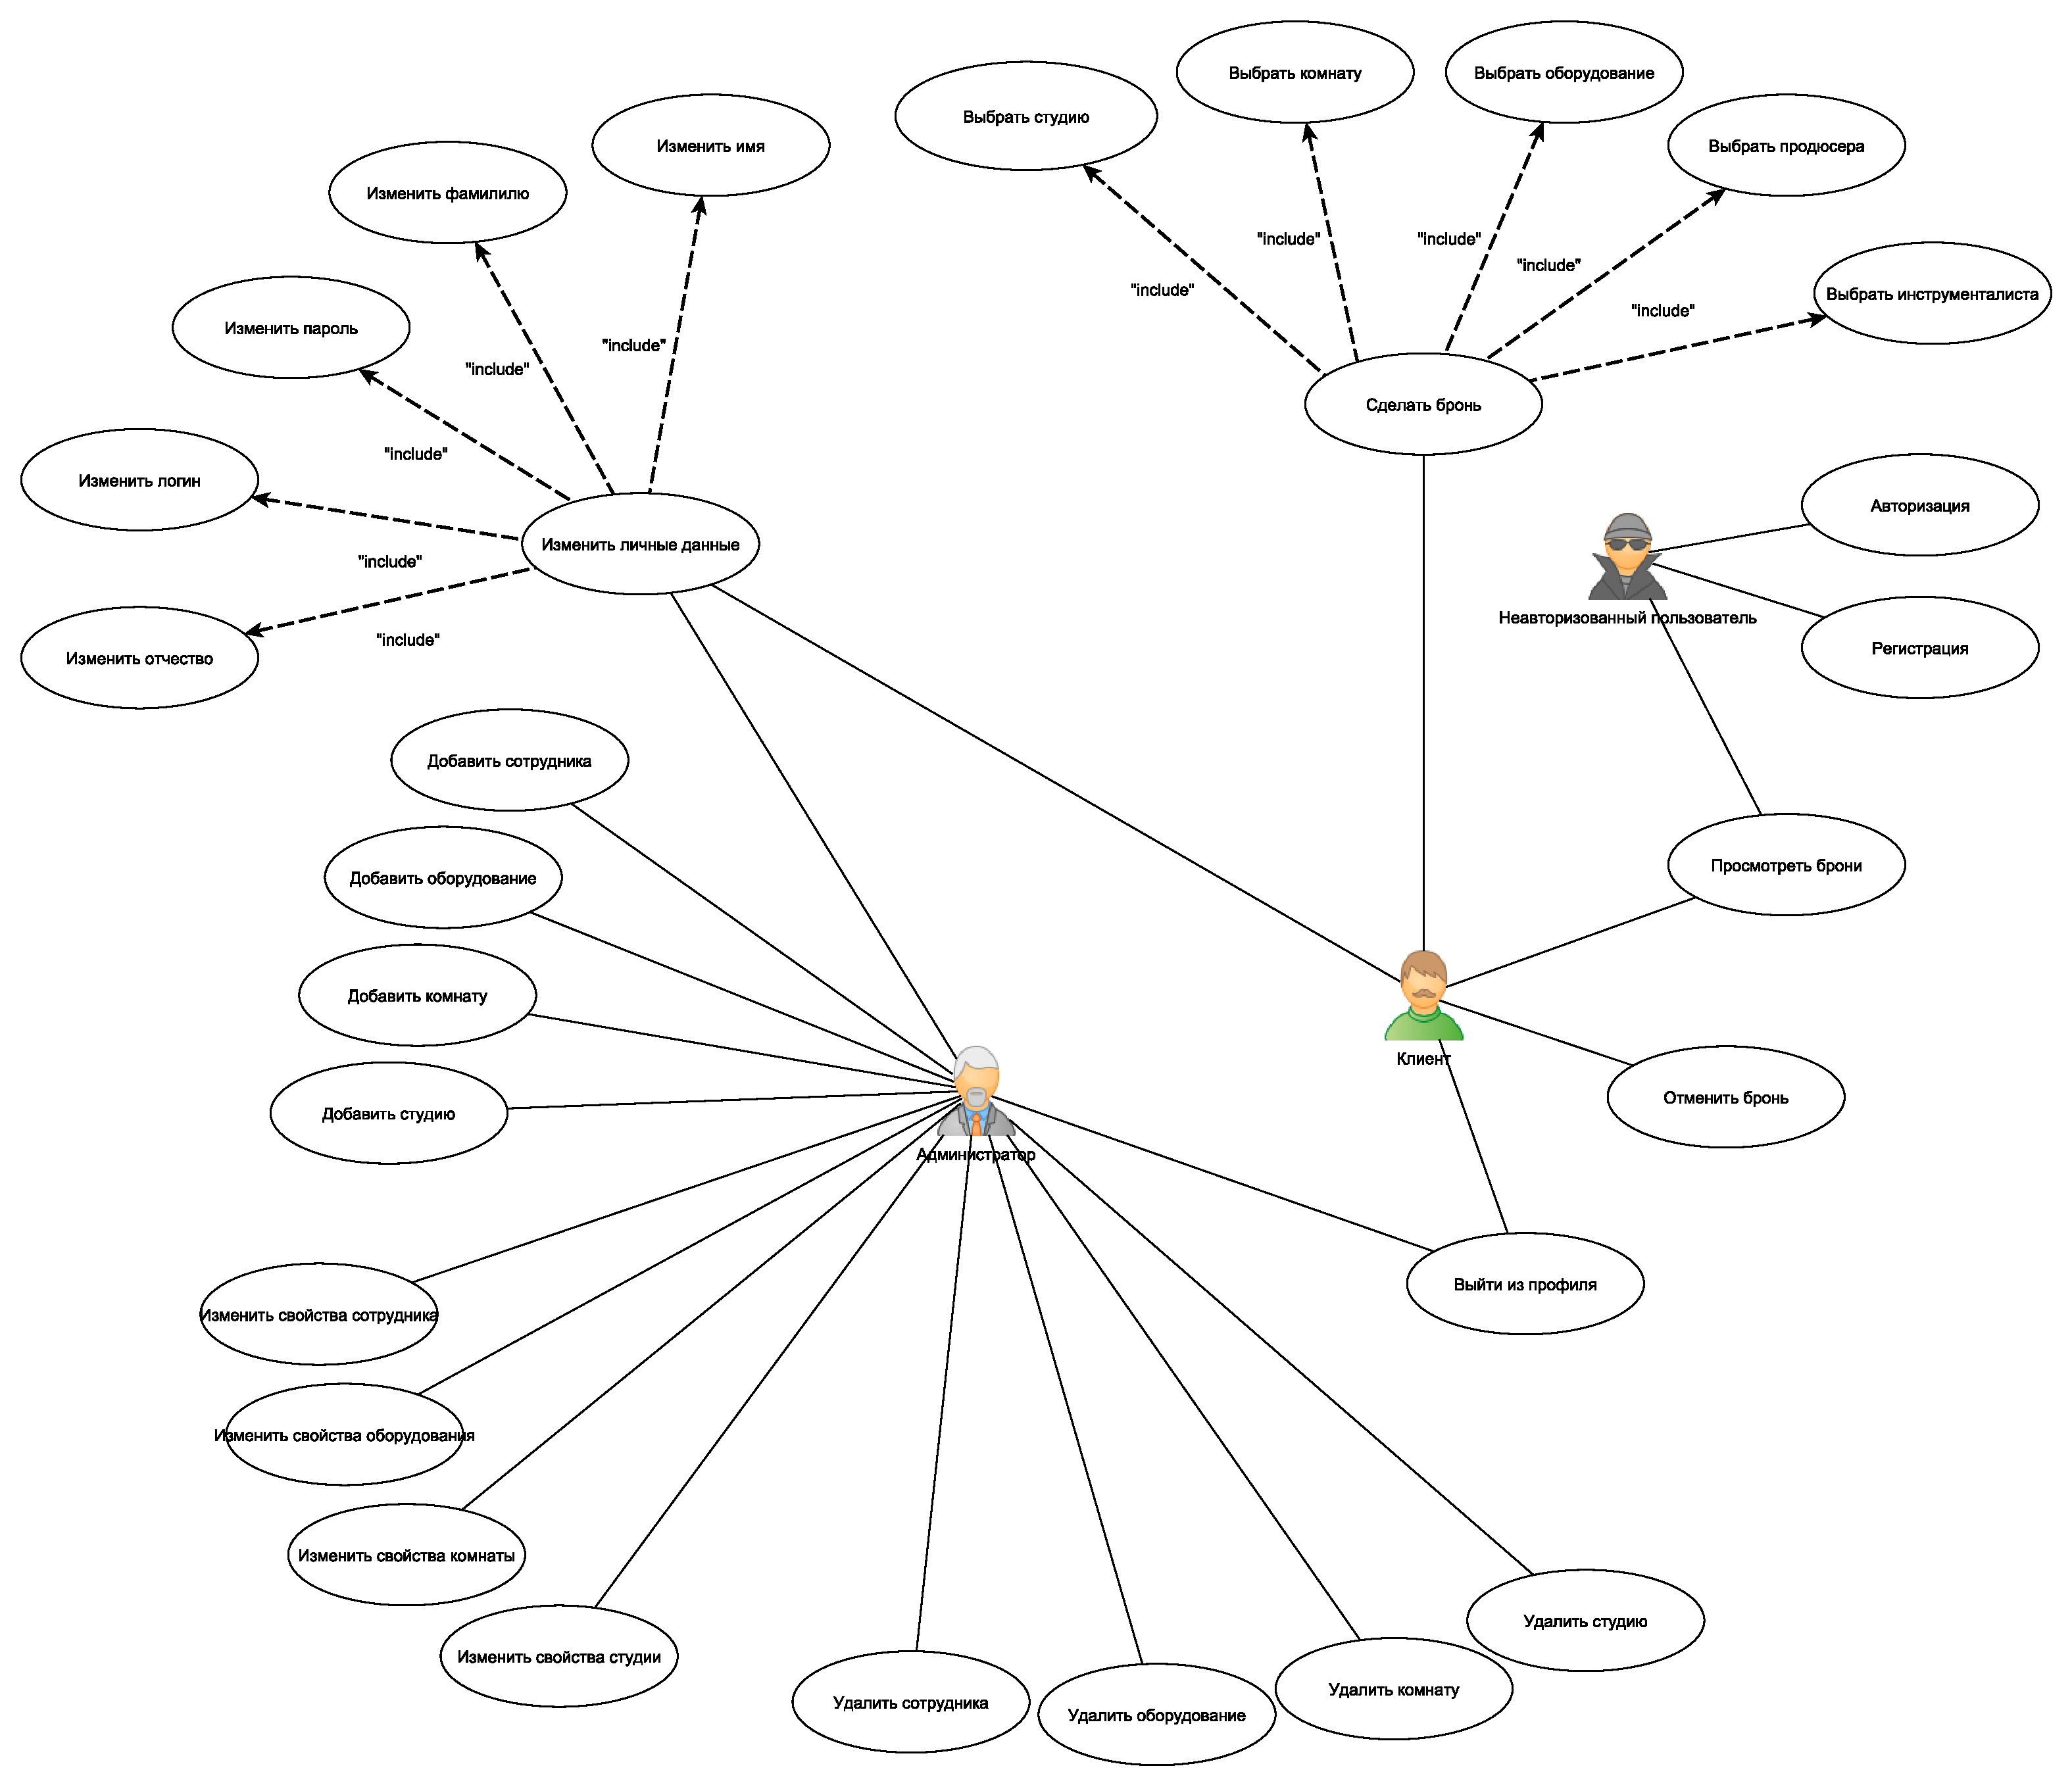
\includegraphics[height=0.55\textheight]{inc/img/use_case.pdf}
%	\captionof{figure}{Пользовательские сценарии}
%	\label{img:use_case}
%\end{center}

\includeimage
{use_case} % Имя файла без расширения (файл должен быть расположен в директории inc/img/)
{f} % Обтекание (с обтеканием)
{H} % Положение рисунка (см. wrapfigure из пакета wrapfig)
{0.9\textwidth} % Ширина рисунка
{Пользовательские сценарии} % Подпись рисунка

% В рамках данной работы необходимо разработать веб приложение, 


\section{Анализ существующих баз данных}
Базы данных по способу хранения делят на две группы --- колоночные и строковые.

\subsection{Колоночные базы данных}
В колоночных базах данных значения одного атрибута хранятся последовательно друг за другом.
Каждая колонка, хранимая на диске, разделена на блоки определенного размера.
Блок состоит из заголовка, размер которого пренебрежительно мал по сравнению с размером блока и непосредственно данных.
Каждой записи в столбце сопоставляется ее позиция (номер строки)~\cite{strokovie_and_kolonochnie_bd}.
\subsection{Строчные базы данных}
Под строчным хранением данных обычно понимается физическое хранение кортежа любого отношения в виде одной записи, в котором значение атрибута идут последовательно одно за другим, а за последним атрибутом кортежа в общем случае следует новый кортеж отношения.
План запроса представляет собой дерево, у каждого узла которого имеется один родитель и один (или два в случае пересечения) дочерних узла
\cite{strokovie_and_kolonochnie_bd}.



\section{Анализ моделей баз данных}
Модель данных --- совокупность структур данных и операций по их обработке \cite{dbms}.

Существуют модели данных следующих типов:
\begin{itemize}
	\item дореляционные;
	\item реляционные;
	\item постреляционные.
\end{itemize}

\subsection{Дореляционные модели}
К дореляционным моделям относят модель инвертированных списков, иерархическую модель и сетевую модель:

\begin{enumerate}
	\item модель инвертированных списков.
	БД на основе модели инвертированных списков представляет собой совокупность файлов, содержащих записи.
	Для записей в файле определен некоторый порядок, диктуемый физический организацией данных.
	Для каждого файла может быть определено произвольное число других упорядоченностей на основании значений некоторых полей записей.
	Обычно для этого используются индексы.
	В такой модели данных отсутствуют ограничения целостности как таковые.
	Все ограничения на возможные экземпляры БД задаются теми программами, которые работают с БД.
	Одно из немногих ограничений, которое может присутствовать --- это ограничение, задаваемое уникальным индексом;
	
	\item иерархическая модель данных строится по принципу иерархии типов объектов, то есть один из типов объекта является главным, а остальные, находящиеся на низших уровнях иерархии, --- подчиненными.
	Между главным и подчиненными объектами устанавливается взаимосвязь <<один~--~ко~--~многим>> \cite{dbms};
	
	\item В сетевой модели данных любой объект может быть и главным, и подчиненным.
	Один и тот же объект может одновременно выступать и в роли владельца, и в роли члена набора.
	Это означает, что любой объект может участвовать в любом числе зависимостей \cite{dbms}.
\end{enumerate}

\subsection{Реляционные модели}
База данных на реляционной модели представляет собой множество отношений.
Множество отношений и операций над ними образуют реляционную алгебру.
Список операций содержит проекцию, выборку, объединение, пересечение, вычитание, соединение и деление \cite{dbms}.

\subsection{Постреляционные модели}
Классическая реляционная модель предполагает неделимость данных, хранящихся в полях записей таблиц.
Это означает, что информация в таблице представляется в первой нормальной форме.
Существует ряд случаев, когда это ограничение мешает эффективной реализации приложений.
Постреляционная модель данных представляет собой расширенную реляционную модель, снимающую ограничение неделимости данных, хранящихся в записях таблиц.
Постреляционная модель данных допускает многозначные поля --- поля, значения которых состоят из подзначений.
Набор значений многозначных полей считается самостоятельной таблицей, встроенной в основную таблицу \cite{voroneg}.
 
\section*{Вывод}
В данном разделе была проанализирована предметная область, проведена формализация задачи, проведена формализация и описание информации, проведена формализация и описание пользователей и проанализированы модели баз данных. 

% \section{Анализ систем управления базами данных}
 
 % про субд https://cyberleninka.ru/article/n/obosnovanie-vybora-modeli-hraneniya-dannyh-dlya-sistemy-monitoringa-kosmicheskogo-prostranstva/viewer